\begin{pa} \label{PA:11.3} A tetrahedron is a three-dimensional figure with four faces, each of which is a triangle. A picture of the tetrahedron $T$ with vertices $(0,0,0)$, $(1,0,0)$, $(0,1,0)$, and $(0,0,1)$ is shown in Figure \ref{F:11.3.Tetrahedron_PA}. If we place one vertex at the origin and let vectors $\va$, $\vb$, and $\vc$ be determined by the edges of the tetrahedron that have one end at the origin, then a formula that tells us the volume $V$ of the tetrahedron is
\begin{equation} \label{eq:11.3.tetrahedron_volume}
V = \frac{1}{6} \lvert \va \cdot (\vb \times \vc) \rvert.
\end{equation}
\begin{figure}[h]
\begin{center}
\begin{minipage}{2.5in}
\begin{center}
  %\resizebox{!}{2.0in}{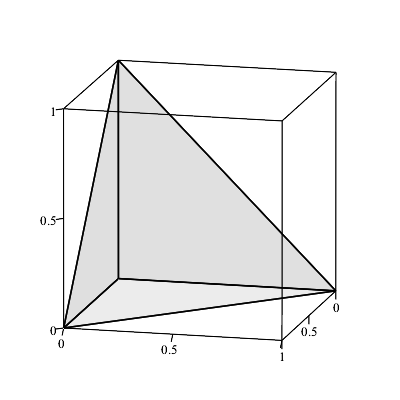
\includegraphics[trim=0.5cm 1.0cm 0.5cm 1.0cm, clip]{11_3_Tetrahedron_PA}} %crop graphics in animate trim=<left> <bottom> <right> <top>, add, clip with \includegraphics
  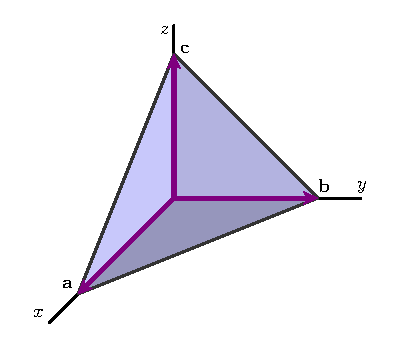
\includegraphics{figures/fig_11_3_tetrahedron.eps}
\end{center}
\caption{The tetrahedron $T$.}
\label{F:11.3.Tetrahedron_PA}
\ \vspace{0.05in} \
\end{minipage} \hspace{0.5in}
\begin{minipage}{2.5in}
\begin{center}
%\resizebox{!}{2.0in}{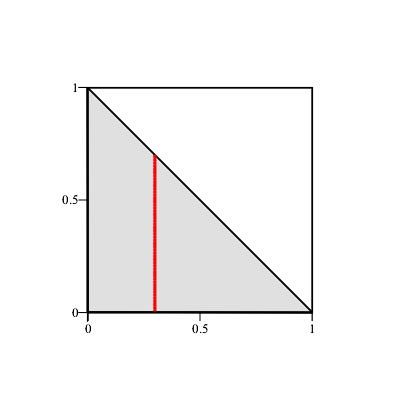
\includegraphics[trim=1.0cm 1.5cm 1.0cm 1.5cm, clip]{11_3_Tetrahedron_proj_PA}} %crop graphics in animate trim=<left> <bottom> <right> <top>, add, clip with \includegraphics
  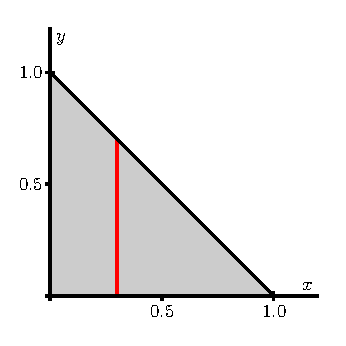
\includegraphics{figures/fig_11_3_tetra_project.eps}
\end{center}
\caption{Projecting $T$ onto the $xy$-plane.}
\label{F:11.3.Tetrahedron_proj_PA}
\end{minipage}
\end{center}
\end{figure}
    \ba
    \item Use the formula (\ref{eq:11.3.tetrahedron_volume}) to find the volume of the tetrahedron $T$.
    
    \item Instead of memorizing or looking up the formula for the volume of a tetrahedron, we can use a double integral to calculate the volume of the tetrahedron $T$. To see how, notice that the top face of the tetrahedron $T$ is the plane whose equation is
        \[z = 1-(x+y).\]
        Provided that we can use an iterated integral on a non-rectangular region, the volume of the tetrahedron will be given by an iterated integral of the form
        \[\int_{x=?}^{x=?} \int_{y=?}^{y=?} 1-(x+y) \, dy \, dx.\]
        The issue that is new here is how we find the limits on the integrals; note that the outer integral's limits are in $x$, while the inner ones are in $y$, since we have chosen $dA = dy \, dx$. To see the domain over which we need to integrate, think of standing way above the tetrahedron looking straight down on it, which means we are projecting the entire tetrahedron onto the $xy$-plane. The resulting domain is the triangular region shown in Figure \ref{F:11.3.Tetrahedron_proj_PA}. \\

Explain why we can represent the triangular region with the inequalities
        \[0 \leq y \leq 1-x \ \ \ \text{ and } \ \ \ 0 \leq x \leq 1.\]
        (Hint: Consider the cross sectional slice shown in Figure \ref{F:11.3.Tetrahedron_proj_PA}.)


\item Explain why it makes sense to now write
the volume integral in the form
        \[\int_{x=?}^{x=?} \int_{y=?}^{y=?} 1-(x+y) \, dy \, dx = \int_{x=0}^{x=1} \int_{y=0}^{y=1-x} 1-(x+y) \, dy \, dx. \]

\item Use the Fundamental Theorem of Calculus to evaluate the iterated integral
        \[\int_{x=0}^{x=1} \int_{y=0}^{y=1-x} 1-(x+y) \, dy \, dx\]
        and compare to your result from part (a).  (As with iterated integrals over rectangular regions, start with the inner integral.)

    \ea

\end{pa} 


\begin{activitySolution}

    \ba
    \item Let $O=(0,0,0)$, $P=(1,0,0)$, $Q=(0,1,0)$, and $R=(0,0,1)$. With these points as the vertices of the tetrahedron we have
 \[\va = \langle 1,0,0 \rangle, \ \ \ \vb = \langle 0,1,0 \rangle, \ \ \ \text{ and } \ \ \ \vc = \langle 0,0,1 \rangle,.\]
Using the formula we obtain
\begin{align*}
\frac{\va \cdot (\vb \times \vc)}{6} &= \frac{\vi \cdot (\vj \times \vk)}{6} \\
    &= \frac{\vi \cdot \vi}{6} \\
    &= \frac{1}{6}.
\end{align*}


    \item If we take a cross section of the domain for a fixed value of $x$ as shown in Figure \ref{F:11.3.Tetrahedron_proj_PA}, we can see that the $y$ values on the cross section all have a lowest value of 0, but their highest values lie on the line $y=1-x$. We can construct these cross sections for any value of $x$ between 0 and 1, so this triangular region is described by the inequalities $0 \leq y \leq 1-x$ and $0 \leq x \leq 1$.


\item When we slice vertically, each slice runs from the $x$-axis to the line $y=1-x$. So the limits on $y$ are $0 \leq y \leq 1-x$. The triangular region has $x$ values that run from $0$ to $1$, so the limits on the integral as as shown. 

\item Using basic integration techniques we have
\begin{align*}
\int_{0}^{1} \int_{0}^{1-x} 1-(x+y) \, dy \, dx &= \int_0^1 \left(y - xy - \frac{y^2}{2} \right)\biggm|_0^{1-x} \, dx \\
    &= \int_0^1 (1-x) - x(1-x) - \frac{1}{2}(1-x)^2 \, dx \\
    &= \frac{1}{2} \int_0^1 x^2-2x+1 \, dx \\
    &= \frac{1}{2}\left(\frac{x^3}{3} - x^2 + x \right)\biggm|_0^1 \\
    &= \frac{1}{2}\left(\frac{1}{3}\right) \\
    &= \frac{1}{6}.
\end{align*}
This is the same result we obtained from the formula in part (a).


    \ea

\end{activitySolution}

\afterpa 